\chapter{Introduction to Software Security}

\section{Fundamentals of Software Security}
\subsection{Software Requirements and Security}
Good software engineering aims to meet a specific set of requirements, which can be broadly divided into functional and non-functional categories. 
\begin{itemize}
    \item \textbf{Functional requirements} specify what the software must do. They define the intended behavior and the tasks the software is designed to accomplish.
    \item \textbf{Non-functional requirements} specify how the software should perform its tasks. These include usability, performance, reliability, safety, and, crucially, \textbf{security}.
\end{itemize}

Creating inherently secure applications is a fundamental, yet often unknown, skill for a good developer or software engineer. Creating secure software is inherently difficult because security is a negative goal: it is about preventing unwanted behaviors rather than just ensuring desired ones. 

\subsection{Bugs, Vulnerabilities, and Exploits}

\begin{tcolorbox}[colback=blue!5!white,colframe=blue!75!black,title=Exam Insight]
Questions about this topic are usually based on identifying assets at risk, associated threats, threat agents, and assessing vulnerabilities for a given scenario (e.g., floor cleaning robots, tracking devices, infrastructure). You may be asked to analyze vulnerabilities, explain potential exploits, and propose concrete countermeasures to reduce risk. Furthermore, be prepared to suggest potential attack surfaces for a described infrastructure, analyze custom authentication mechanisms to highlight weaknesses (like snooping or guessing), and correct Risk Analysis Tables (Likelihood/Impact) while justifying your changes and selecting the best countermeasures.
\end{tcolorbox}

Software is designed to implement specifications. When these specifications are not met, the software contains flaws.
\begin{itemize}
    \item An unmet functional specification results in a \textbf{software bug}.
    \item An unmet security specification results in a \textbf{vulnerability}.
\end{itemize}

It is important to distinguish between a vulnerability and an exploit. A vulnerability is a weakness in the system, whereas an \textbf{exploit} is a specific method, piece of code, or technique used to leverage a vulnerability to violate a system's security properties (Confidentiality, Integrity, Availability - CIA). 
Therefore, having a vulnerability does not necessarily mean an exploit exists, although it opens the door for one to be developed.

\section{The Vulnerability Lifecycle and Disclosure}

\subsection{The Lifecycle of a Vulnerability}
The life of a software vulnerability can be represented as a timeline of key events, from its introduction into the codebase to its eventual remediation. 

\begin{figure}[hbtp]
\centering
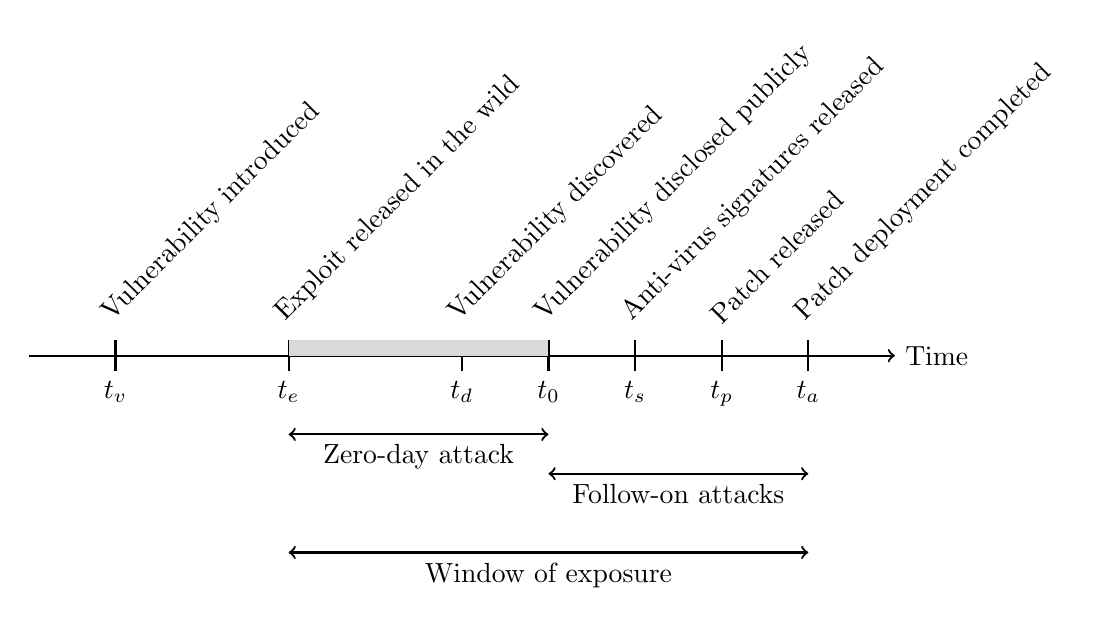
\begin{tikzpicture}[xscale=1.1, yscale=1]
\draw[->, thick] (0,0) -- (10,0) node[right] {Time};

\draw[thick] (1,-0.2) node[below] {$t_v$} -- (1,0.2) node[above, rotate=45, anchor=south west] {Vulnerability introduced};
\draw[thick] (3,-0.2) node[below] {$t_e$} -- (3,0.2) node[above, rotate=45, anchor=south west] {Exploit released in the wild};
\draw[thick] (5,-0.2) node[below] {$t_d$} -- (5,0.2) node[above, rotate=45, anchor=south west] {Vulnerability discovered};
\draw[thick] (6,-0.2) node[below] {$t_0$} -- (6,0.2) node[above, rotate=45, anchor=south west] {Vulnerability disclosed publicly};
\draw[thick] (7,-0.2) node[below] {$t_s$} -- (7,0.2) node[above, rotate=45, anchor=south west] {Anti-virus signatures released};
\draw[thick] (8,-0.2) node[below] {$t_p$} -- (8,0.2) node[above, rotate=45, anchor=south west] {Patch released};
\draw[thick] (9,-0.2) node[below] {$t_a$} -- (9,0.2) node[above, rotate=45, anchor=south west] {Patch deployment completed};

\draw[<->, thick] (3,-1) -- (6,-1) node[midway, below] {Zero-day attack};
\draw[<->, thick] (6,-1.5) -- (9,-1.5) node[midway, below] {Follow-on attacks};
\draw[<->, thick] (3,-2.5) -- (9,-2.5) node[midway, below] {Window of exposure};

\fill[gray!30] (3,0) rectangle (6,0.2);
\end{tikzpicture}
\caption{The Vulnerability Lifecycle, illustrating the timeline of disclosure and patching.}
\end{figure}

The period between the exploit release ($t_e$) and public disclosure ($t_0$) is particularly dangerous; attacks occurring during this time are known as \textbf{Zero-day attacks}. The overall \textbf{window of exposure} lasts until the patch is widely deployed ($t_a$).

\subsection{Disclosure Policies}
The history of software vulnerabilities is heavily influenced by how they are disclosed to the public. The debate over disclosure policies has evolved over the years:
\begin{itemize}
    \item \textbf{Non-Disclosure:} Keeping the vulnerability secret to prevent exploitation. However, this often leaves users unprotected if malicious actors find the vulnerability independently.
    \item \textbf{Full Disclosure:} Publishing all details of the vulnerability immediately, forcing vendors to patch quickly but also arming attackers with exploit details.
    \item \textbf{Coordinated Disclosure (or Anti-Disclosure in its extreme):} Working with the vendor to release a patch simultaneously with the vulnerability details, minimizing the zero-day window.
\end{itemize}

\subsection{The Economics of Vulnerabilities: Black Markets and Bug Bounties}
With the rise of the internet, a lucrative \textbf{black market} for exploits emerged. Attackers are willing to pay significant amounts for zero-day exploits. To counter this, legitimate organizations and security platforms (e.g., Bugcrowd, HackerOne) introduced \textbf{Bug Bounties}. These programs financially reward security researchers for responsibly disclosing vulnerabilities, providing an economic incentive to report bugs rather than sell them to malicious actors.

\section{Permissions and Privilege Escalation in UNIX}

\subsection{UNIX Process Privileges: RUID, EUID, and SUID}
To understand software vulnerabilities in practice, we examine process privileges in UNIX-like operating systems. In UNIX, every file has an owner. For example, a file might be owned by user \texttt{foo}.

When a user (e.g., \texttt{bar}) executes a program, the resulting process runs with certain user IDs:
\begin{itemize}
    \item \textbf{Real UID (RUID):} Represents the real owner of the process (the user who executed it, i.e., \texttt{bar}).
    \item \textbf{Effective UID (EUID):} The UID used by the operating system for checking access permissions. Normally, the EUID is equal to the RUID.
    \item \textbf{Saved set-user-ID (SUID):} A special permission bit that can be set on an executable file. If an executable has the SUID bit set, the EUID of the process running it is changed to the owner of the file, rather than the user who executed it.
\end{itemize}

For example, if an executable owned by \texttt{root} has the SUID bit set (\texttt{rwsr-xr-x}), and user \texttt{bar} executes it, the process will have an RUID of \texttt{bar} but an EUID of \texttt{root}. This allows the program to perform privileged operations on behalf of the unprivileged user.

\begin{figure}[hbtp]
\centering
\begin{tikzpicture}
\node[draw, rectangle, inner sep=10pt, align=center] (user) {User \texttt{bar}\\RUID: \texttt{bar}};
\node[draw, rectangle, inner sep=10pt, align=center, right=3cm of user] (proc) {Process\\RUID: \texttt{bar}\\EUID: \texttt{root}};
\node[draw, rectangle, inner sep=10pt, align=center, right=3cm of proc] (file) {\texttt{/etc/secret}\\Owner: \texttt{root}\\Perms: \texttt{rwx------}};

\draw[->, thick] (user) -- node[above] {executes SUID root} (proc);
\draw[->, thick] (proc) -- node[above] {read (EUID checked)} (file);
\end{tikzpicture}
\caption{The SUID mechanism allowing an unprivileged user to execute a process with elevated permissions.}
\end{figure}

\subsection{A Practical Vulnerability Example}
Consider a program designed to read a sensitive file (\texttt{/etc/secret}) accessible only by \texttt{root}, process the configuration, and perform some actions. Because it needs to read a root-owned file, the program is compiled and set with the SUID root bit.

\begin{verbatim}
#include <unistd.h>
#include <stdio.h>

int main(int argc, const char *argv[]) {
    FILE *fp;
    char line[1024];
    
    // The process has EUID = root because of the SUID bit
    fp = fopen("/etc/secret", "r"); 
    
    while (!feof(fp)) {
        fgets(line, 1024, fp);
        puts(line);
    }
    fclose(fp);
    return 0;
}
\end{verbatim}

If this program simply reads \texttt{/etc/secret} and prints it, any user executing this SUID binary can read the secret file. If the program was intended to only parse the file and return an "OK" status but instead prints the file contents on a parsing error, an attacker could craft a malicious input or exploit a parsing bug to force the program to reveal the secret file or execute arbitrary code while retaining \texttt{root} privileges.

\subsection{Exploitation and Patching}

\begin{tcolorbox}[colback=blue!5!white,colframe=blue!75!black,title=Exam Insight]
Exam questions often ask you to identify vulnerabilities in C source code (specifically focusing on Buffer Overflows or Format Strings), find the vulnerable lines, explain whether they are exploitable, and propose fixes (such as dropping privileges appropriately or sanitizing inputs). You may also need to describe the steps and assumptions required to write exploits, draw memory stack layouts before and after execution, and analyze the bypass or effect of mitigations like NX, ASLR, or Stack Canaries.
\end{tcolorbox}

The core issue is that the program holds elevated privileges (EUID = \texttt{root}) for longer than necessary, expanding the \textbf{attack surface}. Any bug in the \texttt{parse()} function or subsequent logic can be exploited with root privileges.

To patch this, developers must apply the principle of privilege separation:
\begin{enumerate}
    \item Acquire privileges only when absolutely necessary.
    \item Perform the privileged operation (e.g., opening the file).
    \item \textbf{Drop the privileges definitively} immediately after the operation is complete.
\end{enumerate}

\begin{verbatim}
    // ...
    fp = fopen("/etc/secret", "r");
    
    // Drop privileges: set EUID back to RUID
    setuid(getuid()); 
    
    // Now execute parsing and unprivileged logic
    fgets(line, 1024, fp);
    // ...
\end{verbatim}
By dropping the privileges before parsing the file, even if the parsing logic contains a vulnerability (like a buffer overflow), the exploit will only execute with the unprivileged user's permissions, severely limiting the impact.

\section{Principles of Secure Design}

\subsection{Core Principles}
Designing secure software requires adherence to several fundamental principles:
\begin{itemize}
    \item \textbf{Reduce privileged parts to a minimum:} Minimize the amount of code that runs with elevated privileges.
    \item \textbf{KISS (Keep It Simple, Stupid):} Complexity is the enemy of security. Simple code is easier to audit, test, and secure.
    \item \textbf{Discard privileges definitively:} As shown in the UNIX example, drop elevated privileges (e.g., reverting EUID to RUID) as soon as they are no longer needed.
    \item \textbf{Open design:} Following Kerckhoffs's principle, the security of a system should not rely on the obscurity of its design or implementation. Security through obscurity is not true security.
    \item \textbf{Fail-safe and default deny:} Systems should fail securely. By default, access should be denied, and explicit permission must be granted.
\end{itemize}

\subsection{Secure Development Practices}
In addition to core principles, specific practices should be integrated into the development lifecycle:
\begin{itemize}
    \item \textbf{Handle concurrency carefully:} Concurrency and race conditions (like Time-of-Check to Time-of-Use, TOCTOU) are notoriously tricky to secure and often lead to vulnerabilities.
    \item \textbf{Avoid risky resources:} Do not use unsafe shared resources (like \texttt{mktemp} in shared directories) or unknown, untrusted third-party libraries.
    \item \textbf{Filter input and output:} Never trust user input. Validate, sanitize, and filter all data entering and leaving the system.
    \item \textbf{Use trusted cryptography:} Do not write your own cryptographic primitives, password hashing, or secret management code. Use well-established, audited libraries.
    \item \textbf{Use trustworthy Random Number Generators (RNGs):} Rely on secure sources of randomness, such as \texttt{/dev/urandom} or \texttt{/dev/random} in UNIX-like systems.
\end{itemize}

\section{Conclusion and Future Topics}
In conclusion, it is crucial to recognize that \textbf{bug-free software does not exist}, and achieving vulnerability-free software is exceedingly difficult. Not all bugs lead to vulnerabilities, and not all vulnerabilities currently have working exploits, but the risk remains.

In subsequent chapters, we will explore specific examples of insecure programming in depth:
\begin{itemize}
    \item \textbf{Memory errors in desktop applications:} Buffer overflow bugs and format string bugs.
    \item \textbf{Code-injection bugs in web applications:} SQL injection (SQLi), Cross-Site Scripting (XSS), and Cross-Site Request Forgery (CSRF).
\end{itemize}

\section*{Chapter Summary}
This chapter introduces the fundamental concepts of software security, distinguishing between bugs, vulnerabilities, and exploits. It covers the vulnerability lifecycle, disclosure policies, and the economics of exploits. It also examines UNIX process privileges (RUID, EUID, SUID) as a practical example of vulnerabilities, highlighting privilege separation and dropping. Finally, it outlines core principles of secure design and development practices.

\begin{table}[hbtp]
\centering
\begin{tabular}{|l|p{10cm}|}
\hline
\textbf{Concept} & \textbf{Description} \\
\hline
\textbf{Software Bug} & An unmet functional specification. \\
\hline
\textbf{Vulnerability} & An unmet security specification (a weakness in the system). \\
\hline
\textbf{Exploit} & A method or code used to leverage a vulnerability to violate security properties. \\
\hline
\textbf{Zero-day Attack} & An attack that occurs between the release of an exploit and the deployment of a patch. \\
\hline
\textbf{SUID (UNIX)} & A permission bit that changes the Effective UID of a process to the file owner's UID. \\
\hline
\textbf{Secure Design} & Core principles like keeping it simple, minimizing privileges, failing securely, and open design. \\
\hline
\end{tabular}
\caption{Key Software Security Concepts}
\end{table}
